%! Author = lazza
%! Date = 11/04/2022

\section{Pipeline}\label{sec:pipeline}

\subsection{MIPS}\label{subsec:heterogeneous-systems}
The MIPS architecture is based on the SIMD model, the instruction set (ISA) is based on 32-bit format instruction.
\begin{figure}[h]
    \centering
    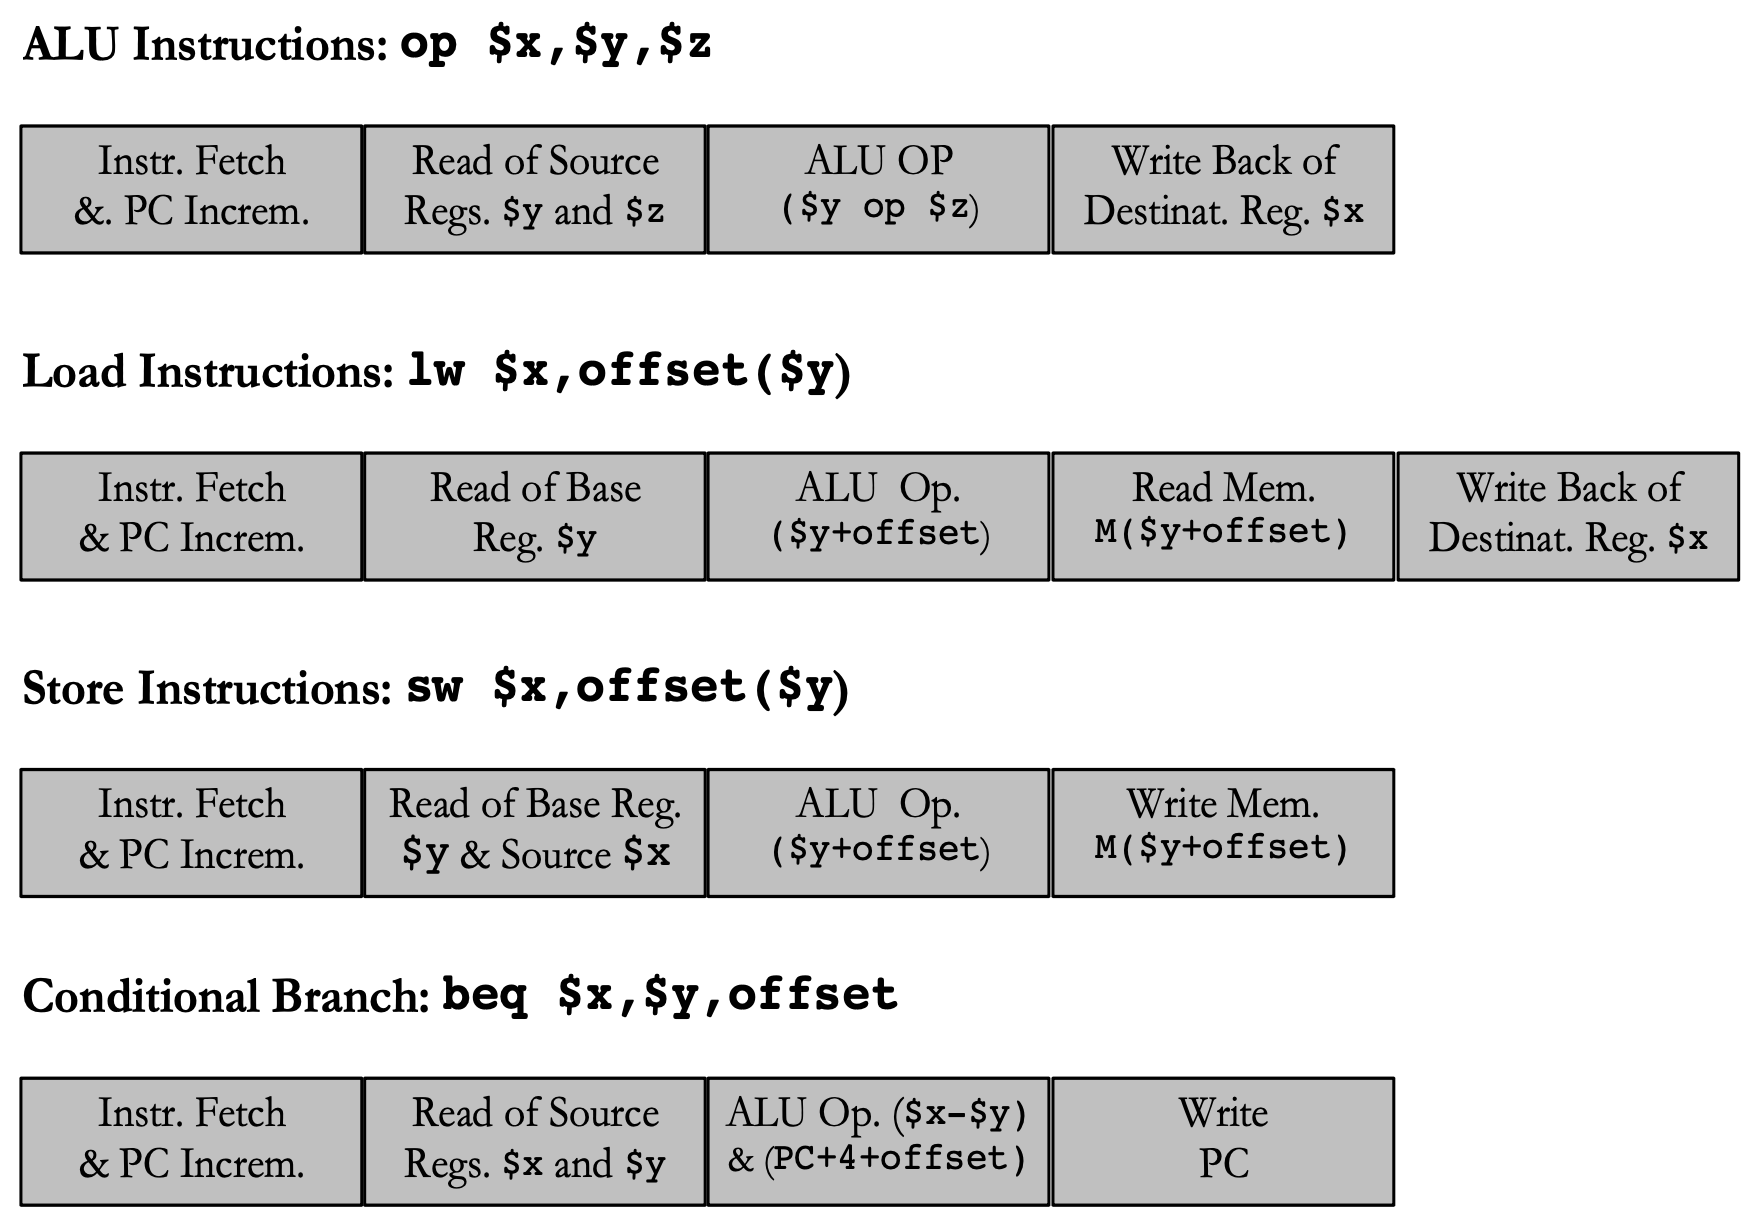
\includegraphics[scale=0.3]{images/MIPS-instructions}
    \caption{MIPS instructions}
    \label{fig: MIPS instructions}
\end{figure}

The CPU, central process unit, amounts to a control unit plus a data path.
Communication between the CPU and the memory in the computing infrastructure happens through the control, data and
address buses.

\begin{figure}[h]
    \centering
    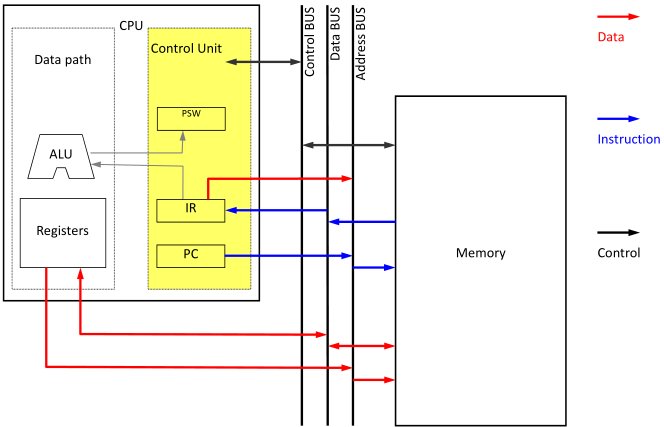
\includegraphics[scale = 0.3]{images/computing-infrastructure}
    \caption{Computing infrastructure}
    \label{fig:computing-infrastructure}
\end{figure}

\paragraph{Execution of MIPS instructions} Every instruction in MIPS subset can be implemented in at most 5 clock
cycles as follows:
\begin{description}
    \item[IF] Instruction Fetch Cycle\\
        Send the content of Program Counter register to Instruction Memory and fetch the
        current instruction from Instruction Memory.

        Update the PC to the next sequential address by adding 4 to the PC (since each instruction is 4 bytes).

    \item[ID] Instruction Decode and Register Read Cycle\\
        Decode the current instruction (fixed-field decoding)
        and read from the Register File of one or two registers
        corresponding to the registers specified in the
        instruction fields.

        Sign-extension of the offset field of the instruction in
        case it is needed.

    \item[EX] Execution Cycle\\
    The ALU operates on the operands prepared in the
    previous cycle depending on the instruction type:
    \begin{itemize}
        \item[-] Register-Register ALU Instructions: ALU executes the specified operation on the operands read
        from the RF
        \item[-] Register-Immediate ALU Instructions:
        ALU executes the specified operation on the first operand
        read from the RF and the sign-extended immediate operand
        \item[-] Memory Reference:
        ALU adds the base register and the offset to calculate the
        effective address.
        \item[-] Conditional branches:
        Compare the two registers read from RF and compute the
        possible branch target address by adding the sign-
        extended offset to the incremented PC\@.
    \end{itemize}


    \item[ME] Memory Access\\
        Load instructions require a read access to the Data
        Memory using the effective address.

        Store instructions require a write access to the Data
        Memory using the effective address to write the data
        from the source register read from the RF\@.

        Conditional branches can update the content of the PC
        with the branch target address, if the conditional test
        yielded true.

    \item[WB] Write-Back Cycle\\
        Load instructions write the data read from memory in
        the destination register of the RF\@.

        ALU instructions write the ALU results into the
        destination register of the RF\@.
\end{description}


\begin{figure}[h]
    \centering
    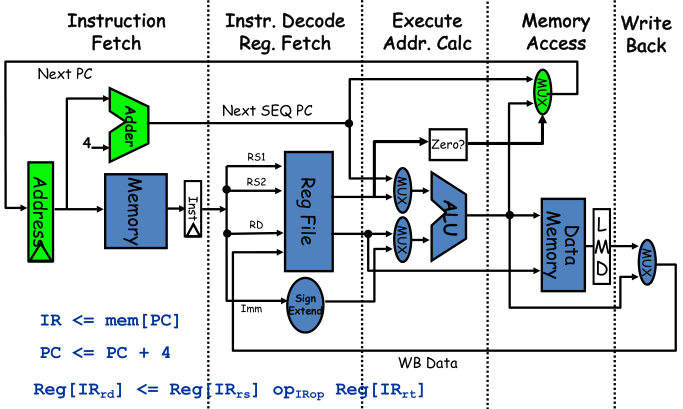
\includegraphics[scale = 0.35]{images/MIPS-data-path}
    \caption{MIPS data path}
    \label{fig:mips-data-path}
\end{figure}

In the single cycle implementation of MIPS the length of the clock cycle is defined by the critical path given by the
load instruction: T = 8ns.
Each instruction is executed in a single clock cycle of 8ns.
\begin{figure}[h]
    \centering
    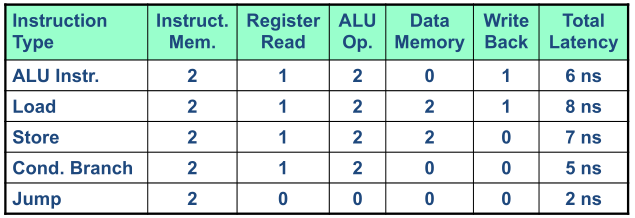
\includegraphics[scale=0.38]{images/instructions-latency}
    \caption{Instruction latency}
    \label{fig:instruction-latency}
\end{figure}

In the multi-cycle implementation the instruction is distributed on multiples cycle (5 for MIPS).

The basic cycle is smaller of 2 ns, the instruction latency is 10 ns.

The multi-cycle execution can be sequential of pipelined.
\begin{figure}[h]
    \centering
    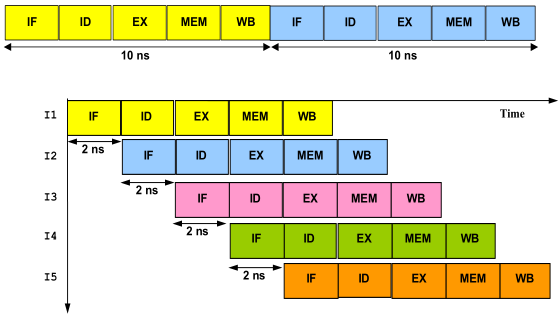
\includegraphics[scale=0.4]{images/sequential-vs-pipelined}
    \caption{Sequential vs pipelined execution}
    \label{fig:sequential-vs-sequential}
\end{figure}

\paragraph{Latency} Each instruction is worsened from 8ns to 10ns.\\
\textbf{Throughput} Is improved by four times, 1 instruction each 8ns to 1 instruction each 2ns.


The Register File is used in WB and ID stages.
In the \textbf{optimized pipeline} the RF-write in the first half of the clock cycle and the RF-read occurs in the
second half of the clock cycle avoiding a possible read after write hazard which otherwise would've required a stall.
It is safely to assume that the optimized pipeline will be the standard pipeline throughout the course.